\chapter{Resoconto delle attività di verifica}
\label{resoconto}
\section{Analisi}\label{Analisi}
Nel periodo antecedente la Revisione dei Requisiti sono stati verificati i documenti ed i processi applicando quanto descritto nelle \normediprogetto.\\
L'analisi statica è stata effettuata secondo i criteri e le modalità indicate nelle \textit{Norme di Progetto}.\\ 
Per gli errori riscontrati effettuando \textit{walkthrough$_{G}$}, si è provveduto a correggere le anomalie riscontrate e sono stati riportati nella lista di controllo nelle \normediprogetto per permettere di effettuare inspection successivamente.\\
L'\textit{inspection$_{G}$} viene effettuata utilizzando la lista di controllo precedentemente stilata. \\
Si sono poi calcolate le metriche descritte nelle \textit{Norme di Progetto}.\\
L'avanzamento dei processi viene poi valutato secondo le metriche descritte nelle \textit{Norme di Progetto}. 
\subsection{Verifica dei processi}
Per il\glossario{processo}di stesura dei documenti, il calcolo delle metriche di Budget Variance e di Schedule Variance è stato effettuato sul valore complessivo delle ore impiegate dal totale dei componenti del gruppo.\\
Per le successive fasi del \textit{progetto$_{G}$}, il gruppo si propone di automatizzare il processo di calcolo delle ore impiegate, con il dettaglio puntuale dei singoli processi.
Lo Schedule Variance totale è di -1 ore e il Budget Variance totale equivale a -25\euro.
\begin{comment}
\begin{tabularx}{\textwidth}{|C|C|C|}
	\hline
	\textbf{Macro-Attività}& \textbf{SV}&\textbf{BV}\\
	\hline
	\textit{Norme di Progetto}    & \euro & \euro\\
	\textit{Piano di Progetto}    & \euro & \euro\\
	\textit{Studio di Fattibilità} & \euro & \euro\\
	\textit{Analisi dei Requisiti}& \euro & \euro\\
	\textit{Piano di Qualifica}   & \euro & \euro\\
	\textit{Glossario}            & \euro & \euro\\
	\hline
	\caption{Esito verifica processi}
\end{tabularx}
\end{comment}

\subsection{Verifica dei documenti}
\begin{tabularx}{\textwidth}{|C|c|C|}
	\hline
	\textbf{Documento}& \textbf{Indice di Gulpease}&\textbf{Esito}\\
	\hline
	\endhead
	\textit{Norme di Progetto}    & 76 & Superato \\
	\textit{Piano di Progetto}    & 64 & Superato \\
	\textit{Studio di Fattibilità} & 61 & Superato\\
	\textit{Analisi dei Requisiti}& 80 & Superato \\
	\textit{Piano di Qualifica}   & 67 & Superato \\
	\textit{Glossario}            & 68 & Superato \\
	\hline
	\caption{Esito della verifica documenti}
\end{tabularx}

\section{Revisione Analisi}
\label{revisione}
Durante il breve periodo di Revisione Analisi, il gruppo si è preparato allo sviluppo del POC e ha apportato delle correzione ai documenti, migliorando i propri processi. 
\subsection{Verifica dei processi}
I miglioramenti principali (tutti descritti nelle \normediprogetto) sono stati:
\begin{itemize}
	\item Automatizzato il calcolo delle ore di lavoro integrando\glossario{Harvest}ad \textit{Asana$_{G}$};
	\item Automatizzato il calcolo dell'\textit{Indice di Gulpease$_{G}$}, tramite script;
	\item Se dei documenti contenenti degli errori grammaticali raggiungono la repository, un bot avvisa per email chi ha commesso l'errore e invia una notifica al gruppo.
\end{itemize}

\subsubsection{MP001 Schedule variance}
Durante il periodo di Revisione Analisi si è verificato un aumento del ritardo dello stato del progetto, che dopo un certo punto si è stabilizzato, superando di molto la soglia di ottimalità prestabilita.
\begin{figure} [H]
    \centering
	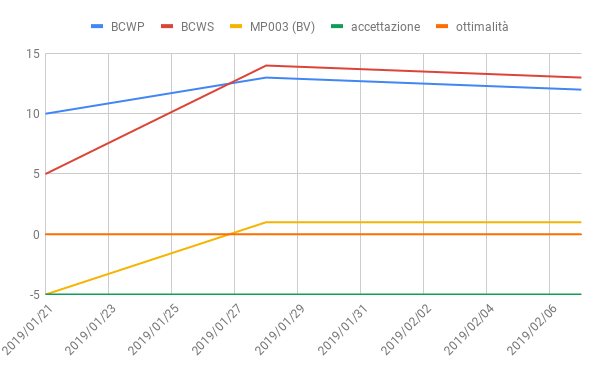
\includegraphics[scale=0.5]{./images/svRa.png}
	\caption{\textit{MP001 - Revisione Analisi}}\label{}
\end{figure}

\subsubsection{MP002 Budget variance}
Con l'aumento dello schedule variance di conseguenza anche il budget variance ha superato di molto le nostre aspettative.
\begin{figure} [H]
    \centering
	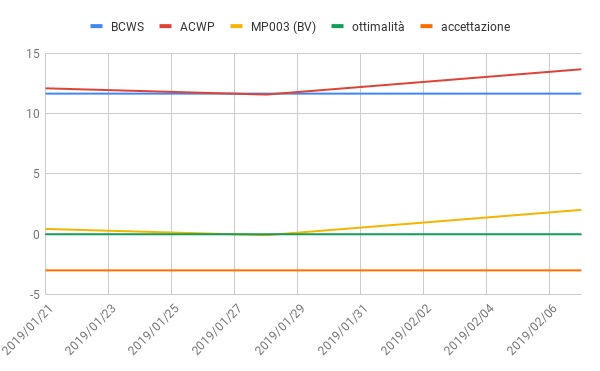
\includegraphics[scale=0.5]{./images/bvra.png}
	\caption{\textit{MP002 - Revisione Analisi}}\label{}
\end{figure}


\section{Progettazione della base tecnologica}
\label{progettazione}
\subsection{MP001: Schedule variance}
A causa di un imprevisto successo all'interno del gruppo con la tecnologia \textit{API}\glossario{Gateway}c'è stato un notevole innalzamento dello schedule variance che ha raggiunto il picco massimo ai primi di marzo.
\begin{figure} [H]
    \centering
	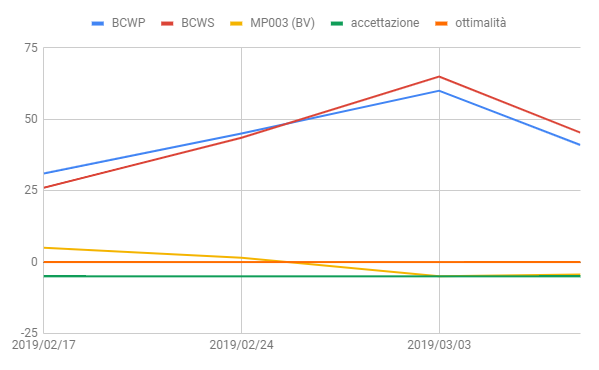
\includegraphics[scale=0.6]{./images/svP.png}
	\caption{\textit{MP001 - Progettazione della base tecnologica}}\label{}
\end{figure}

\subsection{MP002: Budget variance}
In questo periodo il budget variance è stato più o meno sempre stabile ma comunque di molto al di sopra della soglia ottimale.
\begin{figure} [H]
    \centering
	\includegraphics[scale=0.5]{./images/bvP.png}
	\caption{\textit{MP002 - Progettazione della base tecnologica}}\label{}
\end{figure}

\subsection{MP003: SPICE capability level}
Di seguito vengono riportati i livelli di maturità raggiunti dai processi eseguiti durante lo sviluppo del \textit{Proof of Concept$_{G}$}. Data l'inesperienza, non viene raggiunto il livello di accettazione richiesto (3) per la maggior parte dei processi, ma il gruppo sta lavorando per migliorare.
\begin{figure} [H]
    \centering
	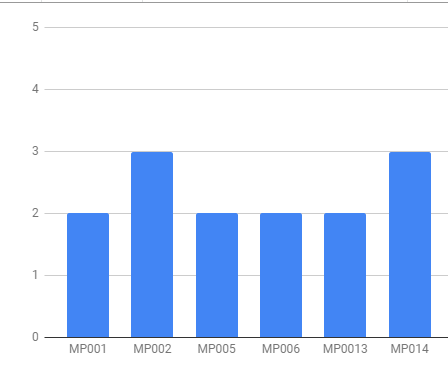
\includegraphics[scale=0.5]{./images/15504.png}
    \caption{\textit{MP003 - ISO/IEC 15504 }}\label{}
\end{figure}

\subsection{MP005:  Occorrenza rischi non previsti}
\textbf{Rischi non previsti: 2}
\begin{itemize}
	\item Un aggiornamento automatico di\glossario{Android Studio}ha completamente rimosso una libreria utilizzata dall'applicazione mobile, quindi il gruppo ha perso tempo per implementane una alternativa. Questo è successo perché la libreria in questione era deprecata. Per evitare problemi simili, l'utilizzo di librerie deprecate è stato vietato, come descritto nelle \textit{Norme di Progetto};
	\item É stata inserita una chiave di accesso Amazon nel repository. Il gruppo è stato avvisato da Amazon, e ha dovuto creare nuove chiavi per tutti i membri.
\end{itemize}

\subsection{MP006: Indisponibilità dei servizi}
\textbf{Indisponibilità dei servizi: 1}\\
Durante il periodo di progettazione della base tecnologica, il gruppo non ha riscontrato problemi riguardanti il downtime di servizi esterni.

\subsection{MP013: Percentuale build superate}
Viene fatta distinzione tra Android e Skill, in quanto vengono contenute in repository diversi.\\
Le build non superate sono 24 su 134 per la Skill e 29 su 232 per Android. Entrambe superano il range di ottimalità (80\%).\\
\begin{figure} [H]
    \centering
	\includegraphics[scale=0.5]{./images/StatobuildTravis-CIandroid.png}
    \caption{\textit{MP013 - Android - Progettazione della base tecnologica}}\label{}
\end{figure}
\begin{figure} [H]
    \centering
	\includegraphics[scale=0.5]{./images/StatobuildTravis-CISkill.png}
    \caption{\textit{MP013 - Skill - Progettazione della base tecnologica}}\label{}
\end{figure}

\subsection{MP014: Media commit giornaliera}
Come si può vedere dai grafici, il numero di commit è stato abbastanza costante, con un aumento del carico di lavoro durante la fine di febbraio.
\begin{figure} [H]
    \centering
	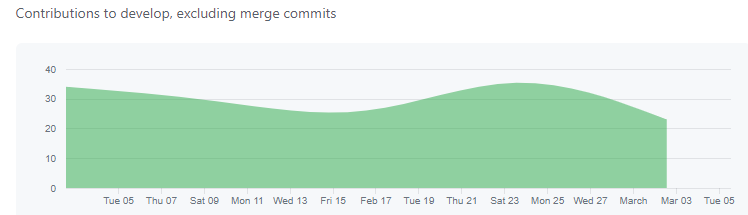
\includegraphics[scale=0.5]{./images/dailycommits_kotlin.PNG}
    \caption{\textit{MP014 - Android - Progettazione della base tecnologica}}
\end{figure}
\begin{figure} [H]
    \centering
	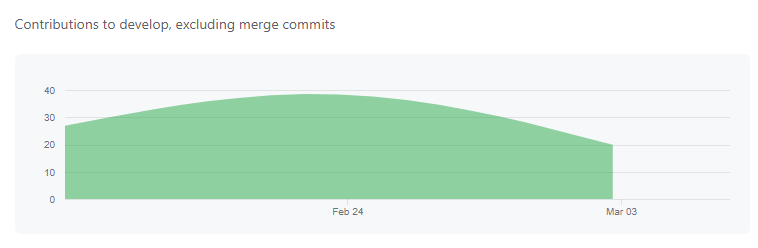
\includegraphics[scale=0.5]{./images/daycommits_js.PNG}
    \caption{\textit{MP014 - Skill - Progettazione della base tecnologica}}
\end{figure}


\subsection{MP015, MP016: Percentuale requisiti soddisfatti}
\begin{figure} [H]
    \centering
	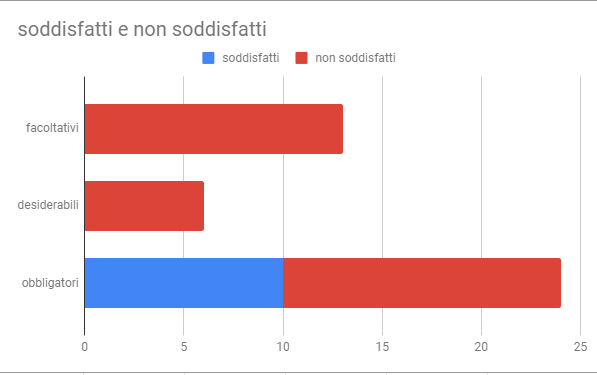
\includegraphics[scale=0.5]{./images/req.PNG}
    \caption{\textit{MP015 - MP016 Tipologia di requisiti}}
\end{figure}
\begin{figure} [H]
    \centering
	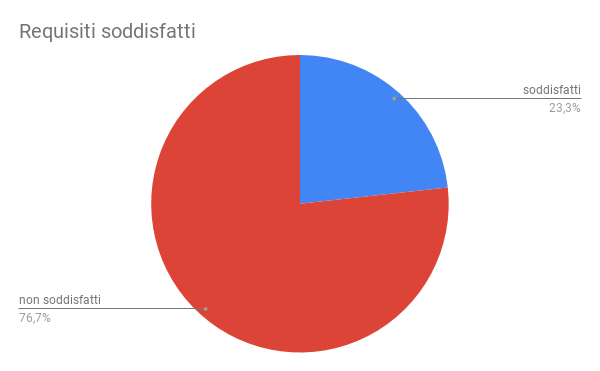
\includegraphics[scale=0.5]{./images/RequisitiSoddisfatti.png}
    \caption{\textit{MP015 - MP016 Differenza soddisfatti e non soddisfatti}}
\end{figure}
\subsection{MPR001 Ortografia}
Grazie allo script per la segnalazione automatica degli errori, questi vengono corretti a ogni push nel develop. Durante la verifica, comunque, sono stati trovati da zero a due errori per documento passati allo script. 
\subsection{MPR002 Indice di Gulpease}
\begin{figure} [H]
    \centering
	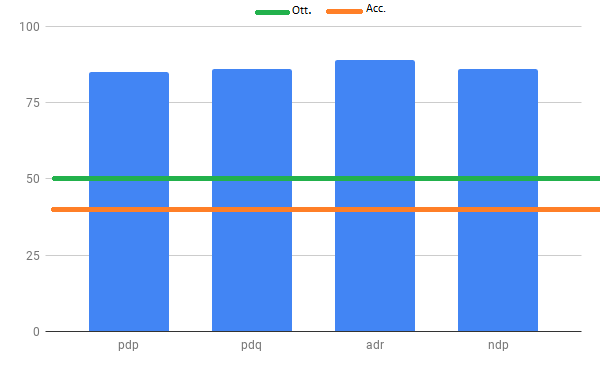
\includegraphics[scale=0.5]{./images/gulpeaseP.png}
    \caption{\textit{MPR002 \textit{Indice di Gulpease$_{G}$}}}
\end{figure}

\section{Progettazione di dettaglio e codifica}
\label{resocontoProg}

\subsection{Revisione complessiva}
Durante il periodo di progettazione di dettaglio e codifica, il gruppo non ha trovato molte difficoltà a svolgere i compiti pianificati. Molte delle attività di codifica sono state supportate da script automatici e tool online attivati nel periodo precedente. C'è stata una buona collaborazione tra i membri del team. Il problema principale si è verificato per l'inesperienza del gruppo sul test driven development, che inizialmente ha rallentato la codifica, ma col tempo questo problema si è ridotto. 

\subsection{MP001: Schedule variance}
\textbf{Passato}\\
La schedule variance è stata abbastanza pertinente con quanto preventivato, questo è dato dal fatto che non ci sono stati seri problemi durante il periodo di Progettazione di dettaglio e codifica.\\
\begin{figure} [H]
    \centering
	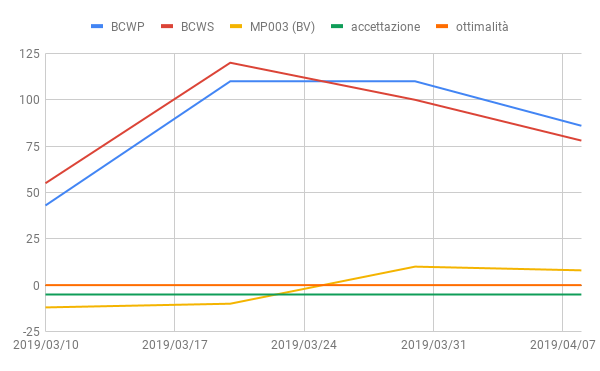
\includegraphics[scale=0.4]{./images/svPDC.png}
	\caption{\textit{MP001 - schedule variance - Progettazione di dettaglio e codifica}}\label{}
\end{figure}

\subsection{MP002: Budget variance}
\textbf{Passato}\\
L'andamento della budget variance rispetta quello della schedule variance.\\
\begin{figure} [H]
    \centering
	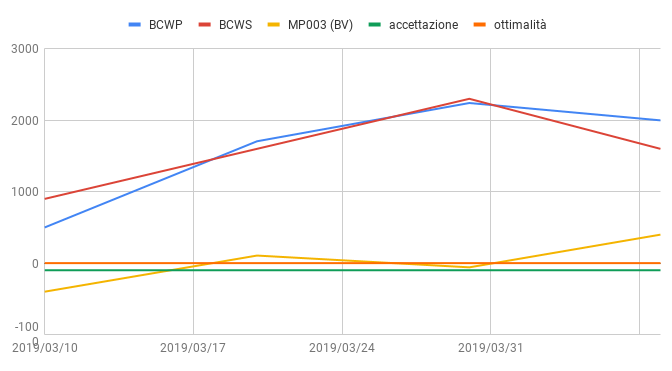
\includegraphics[scale=0.5]{./images/bvPDC.png}
	\caption{\textit{MP002 - budget variance - Progettazione di dettaglio e codifica}}\label{}
\end{figure}
\subsection{MP003: SPICE capability level}
\textbf{Passato 4/6}
\begin{itemize}
	\item \textbf{QP001:} Il gruppo è migliorato sulla Pianificazione dall'inizio del progetto. Dato che tutti hanno svolto almeno una volta ogni ruolo, onguno riesce a svolgere il suo compito. Se questo risulta più difficile di quanto pinificato, la persona in difficoltà crea un ticket su Asana o su Slack così gli altri membri del gruppo possono aiutarlo. Il responsabile riesce a controllare l'andamento del lavoro guardando Asana e le build su travis, senza dover aspettare una risposta da un collega;
	\item \textbf{QP002:} Il miglioramento delle attività di processo risulta ancora qualcosa di complesso da gestire. Questo richiede, nella maggior parte dei casi, una riunione con tutti i membri del gruppo, per prendere una decisione. Questo porta, spesso, alla modifica di un documento e comporta l'apprendimento del nuovo metodo. Detto questo, sono stati fatti alcuni miglioramenti preventivi avvenuti con successo, come per esempio il passaggio a typescript:
		\begin{itemize}
			\item il team si è accorto che la produzione di codice per la backend risultava ostica usando javascript;
			\item il responsabile ha programmato una riunione, nella quale sono stati discussi vantaggi del nuovo linguaggio, facilità per la traduzione (js -> ts), compatibilità con il codice già prodotto;
			\item il team ha deciso di utilizzare TypeScript; 
			\item La traduzione è avvenuta in un paio d'ore e la velocità di produzione delle classi per la Skill è aumentata;
		\end{itemize} 
	\item \textbf{QP003:} I rischi sono mitigati dal fatto che il gruppo è composto da 7 membri, quindi, se qualcuno ha delle difficoltà a svolgere il proprio lavoro, è facile che un altro membro del gruppo sia disposto ad aiutarlo;
	\item \textbf{QP004:} La verifica del software risulta abbastanza semplice, dato che più membri del gruppo hanno esperienza (scolastica) nella produzione di test di unità e integrazione. Questo è supportato dal tool Travis-CI e dalla abbondante documentazione per i test su Node.js. Risulta però ancora ostico lavorare usando il Test Driven Development;
	\item \textbf{QP005:} I test di sistema, integrazione (lato API Gateway - database) risultano difficili da automatizzare, dato che molti dei tool automatici sono a pagamento. Il compito viene quindi svolto a mano, anche se il gruppo ha deciso di produrre uno script per eseguire test funzionali, entro il periodo di Verifica e Collaudo;
	\item \textbf{QP006:} Il versionamento è completamente automatizzato tramite Travis-CI. Per l' applicazione Android è stato semplice, grazie a Gradle; la Skill, essendo scritta in typescript, ha bisogno di essere compilata in javascript, prima di essere pubblicata su AWS Lambda. \\Questo genera molti file .js che sporcano l'ambiente di lavoro. Per risolvere il problema, il gruppo ha prodotto degli script che si occupano di fare pulizia prima di trasferire i file su Github, e per fare il deploy automatico su AWS Lambda.
\end{itemize}
Di seguito viene riportata la tabella con il nome di ogni processo associato al suo codice per facilitare la lettura del grafico:
\begin{itemize}
	\item QP001: Pianificazione delle attività di progetto, valutazione e controllo dei processi \S\ref{pro1};
	\item QP002: Miglioramento continuo delle attività di processo \S\ref{pro2};
	\item QP003: Analisi e prevenzione dei rischi \S\ref{pro3};
	\item QP004: Verifica del software \S\ref{pro4};
	\item QP005: Gestione dei test \S\ref{pro5};
	\item QP006: Versionamento e build \S\ref{pro6}.
\end{itemize}
\begin{figure}[H]
    \centering
	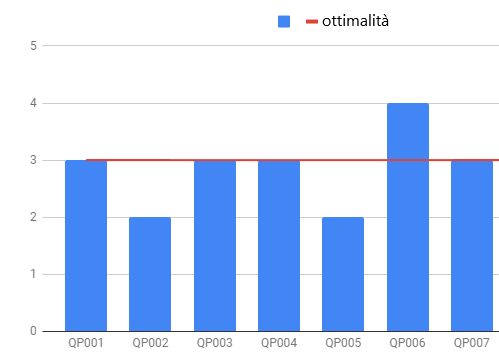
\includegraphics[scale=0.7]{./images/spicePDC.png}
    \caption{\textit{MP003 - ISO/IEC 15504 - Progettazione di dettaglio e codifica}}
\end{figure}

\subsection{MP005:  Occorrenza rischi non previsti}
\textbf{Passato}\\
\textbf{Rischi non previsti: 1}
\begin{itemize}
	\item \textbf{JavaScript:} grazie allo sviluppo del POC durante il periodo di Progettazione della base tecnologica, il gruppo si è accorto di come JavaScript fosse un ostacolo nella produzione della Skill, data la mancanza delle caratteristiche base dei linguaggi di programmazione (principalmente interfacce e tipi di ritorno). Per questo motivo è stato fatto il passaggio a TypeScript all'inizio del periodo di Progettazione di dettaglio e codifica. 
\end{itemize}

\subsection{MP006: Indisponibilità dei servizi}
\textbf{Passato}\\
\textbf{Indisponibilità dei servizi: 0}\\
Durante il periodo di progettazione di dettaglio e codifica, PragmaDB ha avuto qualche giorno di downtime per non sforare con il piano gratuito di Amazon AWS. Questo non ha creato problemi, perché avevamo pieno controllo sul server su cui è hostato. \\

\subsection{MP007 MP008 MP009 MP010 MP011 }
\textbf{Passato}\\
Queste metriche sono state usate per calcolare la manuntenibilità del codice, grazie alla piattaforma di test statici SonarCloud. Questo permette di visualizzare la qualità del software in un solo grafico ricco di informazioni.\\
Il seguente grafico presenta nelle ascisse le linee di codice, nelle ordinate il tempo previsto di risoluzione del problema, la grandezza del cerchio indica la quantità di linee di codice e il colore del cerchio corrisponde alla gravità del problema.\\
Tutti i problemi non in verde sono stati risolti, in quanto indicano un possibile errore grave durante l'esecuzione del codice. Quelli in verde verranno risolti durante il periodo di Verifica e Collaudo.\\
\begin{figure} [H]
    \centering
	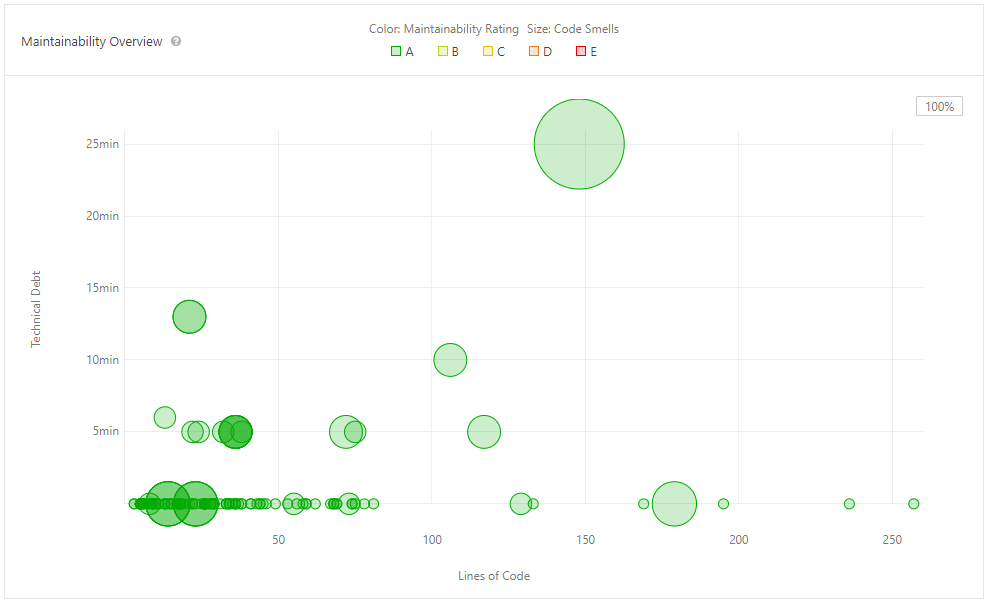
\includegraphics[scale=0.5]{./images/manPDC.png}
    \caption{\textit{MP007 MP008 MP009 MP010 MP011 - manuntenibilità del codice app Android - Progettazione di dettaglio e codifica}}\label{}
\end{figure}
\begin{figure} [H]
    \centering
	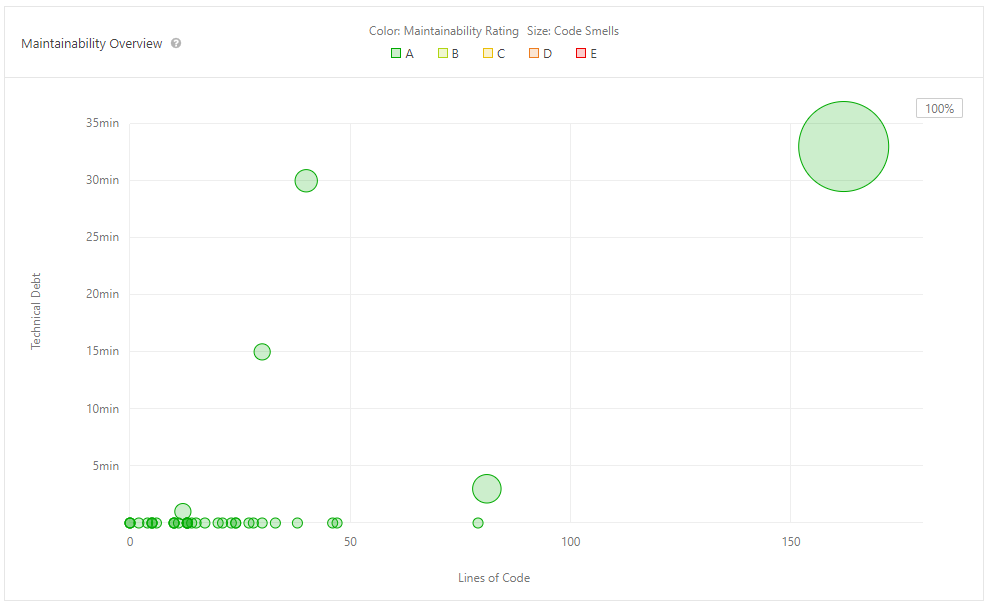
\includegraphics[scale=0.5]{./images/manSPDC.png}
    \caption{\textit{MP007 MP008 MP009 MP010 MP011 - manuntenibilità del codice Skill - Progettazione di dettaglio e codifica}}\label{}
\end{figure}

\subsection{MP011: Tempo medio per risolvere un errore} 
\textbf{Passato}\\
\textbf{tempo medio per risolvere un errore: 33.16 minuti.}\\
La risoluzione degli errori nella Skill risulta molto lunga, in quanto bisogna fare ogni volta il deploy su AWS Lambda per testare le funzioni della skill (richiede da 40 secondi a 2 minuti). Per questo motivo, il team pone molta cura nella redazione dei test di unità e integrazione (che possono essere eseguiti senza deploy).
\begin{figure} [H]
    \centering
	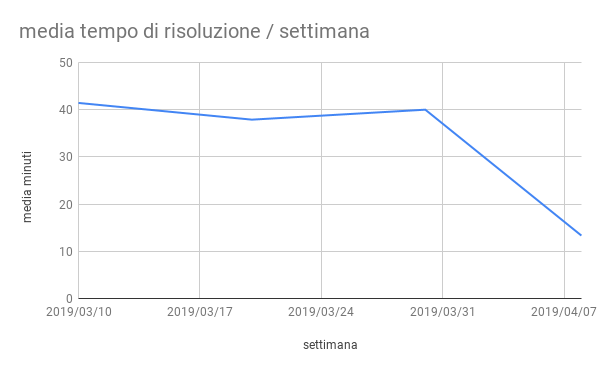
\includegraphics[scale=0.5]{./images/risPDC.png}
    \caption{\textit{MP013 - Skill - Progettazione di dettaglio e codifica}}\label{}
\end{figure}

\subsection{MP012: Efficienza della progettazione dei test}
\textbf{Passato}\\
\textbf{tempo medio per sviluppare un test: 35 minuti.}\\
La progettazione di ogni test velocizza la seguente, in quanto hanno molti punti in comune tra di loro. Questo permette di velocizzare complessivamente la stesura dei test.
\begin{figure} [H]
    \centering
	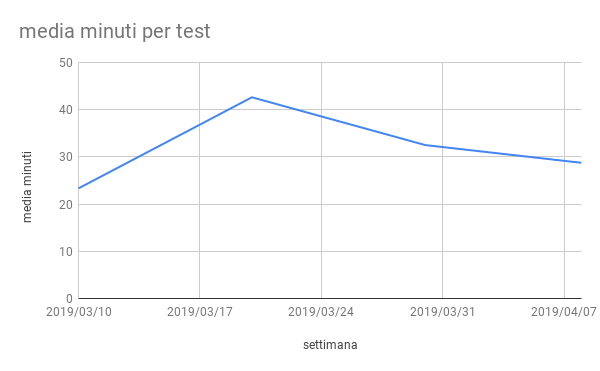
\includegraphics[scale=0.4]{./images/mediatestPDC.png}
    \caption{\textit{MP013 - media minuti per test - Progettazione di dettaglio e codifica}}\label{}
\end{figure}

\subsection{MP013: Percentuale build superate}
\textbf{Passato}\\
Viene fatta distinzione tra Android e Skill, in quanto vengono contenute in repository diversi.\\
Le build dell'applicazione Android sono state per la maggior parte positive. \\
\begin{figure} [H]
    \centering
	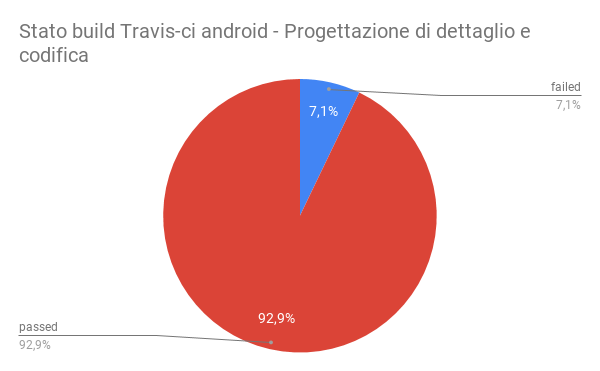
\includegraphics[scale=0.4]{./images/buildandroidPDC.png}
    \caption{\textit{MP013 - Android - Progettazione di dettaglio e codifica}}\label{}
\end{figure}
Le build della Skill (progetto node.js) risultano con molti errori. Questo è dovuto al fatto che sono stati sviluppati test di unità e integrazione prima di produrre il codice. Per questo motivo questa metrica è considerata come passata.\\
\begin{figure} [H]
    \centering
	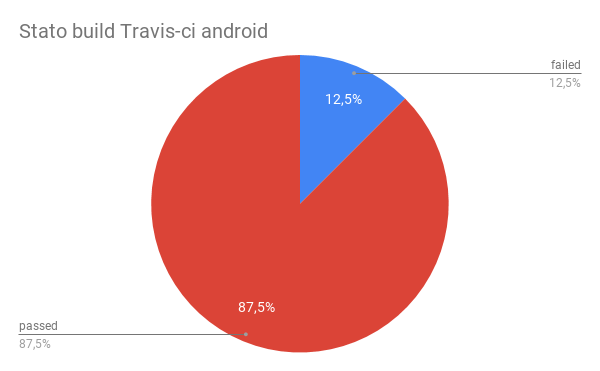
\includegraphics[scale=0.4]{./images/buildPDC.png}
    \caption{\textit{MP013 - Skill - Progettazione di dettaglio e codifica}}\label{}
\end{figure}

\subsection{MP014: Media commit giornaliera}
\textbf{Passato}\\
Il seguente grafico contiene il numero totale di commit giornalieri. Questi risultano poco omogenei, in quanto questo periodo è stato caratterizzato da cicli formati da progettazione di dettaglio (giornate con pochi commit) e codifica (molti commit).\\
\begin{figure} [H]
    \centering
	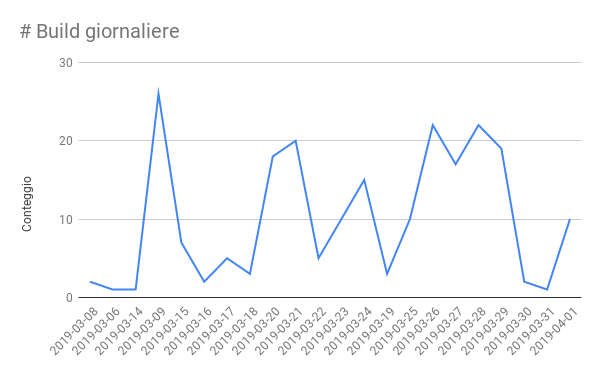
\includegraphics[scale=0.4]{./images/buildsPDC.png}
    \caption{\textit{MP014 numero commit giornalieri - Progettazione di dettaglio e codifica}}
\end{figure}

\subsection{MP015, MP016: Percentuale requisiti soddisfatti}
\textbf{Passato}\\
Sono stati soddisfatti tutti i requisiti che il gruppo aveva preventivato per il periodo di progettazione di dettaglio e codifica, con l'eccezione del requisito riguardante la sveglia, che attualmente non è possibile implementare usando le API fornite da Alexa Skill Kit (dopo una riunione con la proponente, e con la sua approvazione,  questo requisito è stato spostato in "facoltativo - non accettato").
Il gruppo ha stimato che i requisiti obbligatori non soddisfatti richiederanno poco lavoro, in quanto presentano aspetti simili ad altri requisiti (sotto il punto di vista della progettazione in dettaglio e codifica). I requisiti desiderabili e facoltativi sono per la maggior parte riguardanti aspetti secondari del prodotto (invece che blocchi), quindi compresi nelle attività di verifica e collaudo.\\
Come richiesto dal committente, molti dei requisiti sono stati scomposti in requisiti più specifici.\\
requisiti facoltativi sono stati non accettati, dato che il team li ha trovati difficili.\\
\begin{figure} [H]
    \centering
	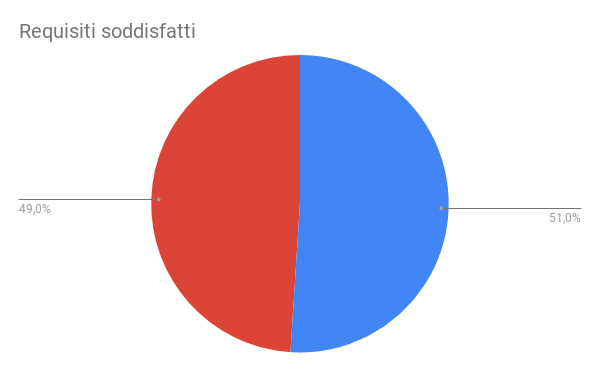
\includegraphics[scale=0.5]{./images/torsodPDC.png}
    \caption{\textit{MP015 - MP016 Tipologia di requisiti - Progettazione di dettaglio e codifica}}
\end{figure}
\begin{figure} [H]
    \centering
	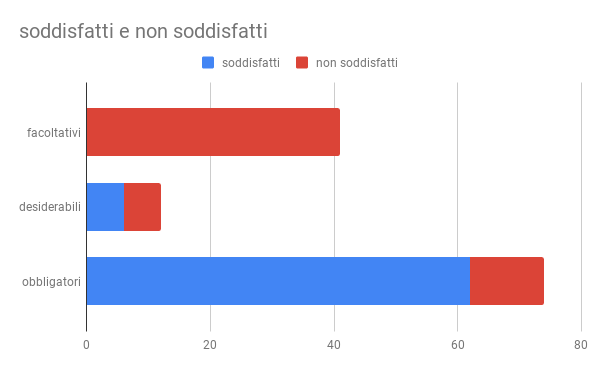
\includegraphics[scale=0.5]{./images/barsodPDC.png}
    \caption{\textit{MP015 - MP016 soddisfatti / non soddisfatti - Progettazione di dettaglio e codifica}}
\end{figure}

\subsection{MPR001 Ortografia}
\textbf{Passato}\\
Gli errori grammaticali trovati durante una ispezione finale sono stati meno di 2 per documento.
\subsection{MPR002 Indice di Gulpease}
\textbf{Passato}\\
Il seguente grafico è stato generato attraverso un bot che calcola giornalmente l'indice di gulpease dei documenti.\\
Si può notare come l'indice di gulpease è sempre stato sopra il limite di accettazione e ottimalità.\\
\begin{figure} [H]
    \centering
	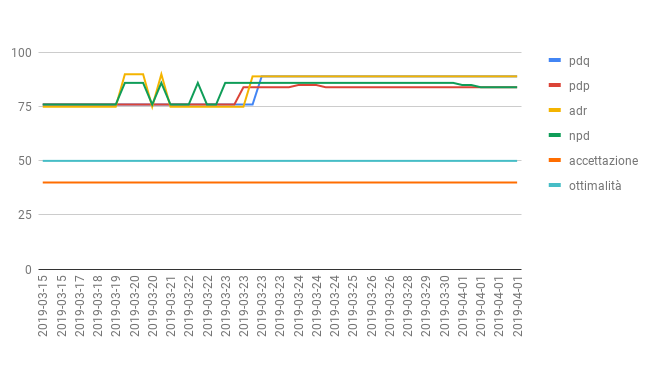
\includegraphics[scale=0.5]{./images/gulpeasePDC.png}
    \caption{\textit{MPR002 \textit{Indice di Gulpease$_{G}$} - Progettazione di dettaglio e codifica}}
\end{figure}


\section{Verifica e collaudo}
Questa sezione verrà compilata alla fine del periodo di Verifica e collaudo.